% !TEX root=./adl.tex

\section{Hyperparameter Selection}

% -----------------------------------------------------------------------
\begin{frame}{Why Hyperparameters Matter}

  Deep learning performance is highly sensitive to hyperparameter choices.
  Poor choices can lead to divergence, slow convergence, or suboptimal generalization.

  \vspace{0.5em}
  \textbf{Key hyperparameters in LLM training:}
  \begin{itemize}
    \item \textbf{Learning rate} and its \emph{schedule} (warmup, decay shape)
    \item \textbf{Batch size} (interacts with learning rate)
    \item \textbf{Weight decay} (regularization strength)
    \item \textbf{Adam parameters} ($\beta_1, \beta_2, \epsilon$)
    \item \textbf{Architectural choices}: depth, width, number of heads
    \item \textbf{Data mix} and \emph{training duration} (tokens seen)
  \end{itemize}

  \vspace{0.5em}
  \textbf{Challenge:} Each training run takes a long time.
  We cannot do grid search over hyperparameters.

  \vspace{0.3em}
  $\Rightarrow$ Need principled, efficient strategies \& insights.
\end{frame}

% -----------------------------------------------------------------------
\subsection{Classical Hyperparameter Optimization}

% -----------------------------------------------------------------------
\begin{frame}{Grid Search vs.\ Random Search}

  \begin{columns}[T]
    \begin{column}{0.52\textwidth}
      \textbf{Grid search:}
      \begin{itemize}
        \item Evaluate all combinations on a regular grid
        \item Cost grows \emph{exponentially} in the number of hyperparameters: $\mathcal{O}(k^d)$
        \item Wastes budget on unimportant dimensions
      \end{itemize}

      \vspace{0.4em}
      \textbf{Random search}~\cite{bergstra2012random}:
      \begin{itemize}
        \item Sample configurations uniformly at random
        \item Each trial explores a \emph{distinct value} for every dimension
        \item Provably more efficient when only a few hyperparameters matter (low effective dimensionality)
        \item Matches or beats grid search using a fraction of the budget
      \end{itemize}
    \end{column}
    \begin{column}{0.44\textwidth}
      \begin{center}
        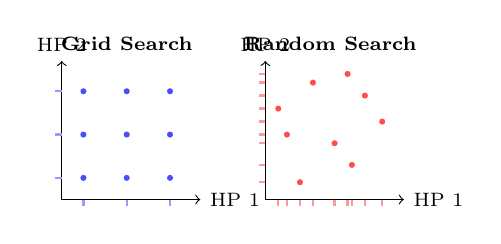
\begin{tikzpicture}[scale=0.55]
          % Grid search
          \begin{scope}[shift={(-0.2,0)}]
            \draw[->] (0,0) -- (3.2,0) node[right, font=\scriptsize] {HP 1};
            \draw[->] (0,0) -- (0,3.2) node[above, font=\scriptsize] {HP 2};
            \node[font=\scriptsize\bfseries] at (1.5,3.6) {Grid Search};
            \foreach \x in {0.5,1.5,2.5} {
              \foreach \y in {0.5,1.5,2.5} {
                \fill[blue!70] (\x,\y) circle (2pt);
              }
            }
            % projections - only 3 unique per axis
            \foreach \x in {0.5,1.5,2.5} {
              \draw[blue!40, thick] (\x,0) -- (\x,-0.15);
            }
            \foreach \y in {0.5,1.5,2.5} {
              \draw[blue!40, thick] (0,\y) -- (-0.15,\y);
            }
          \end{scope}
          % Random search
          \begin{scope}[shift={(4.5,0)}]
            \draw[->] (0,0) -- (3.2,0) node[right, font=\scriptsize] {HP 1};
            \draw[->] (0,0) -- (0,3.2) node[above, font=\scriptsize] {HP 2};
            \node[font=\scriptsize\bfseries] at (1.5,3.6) {Random Search};
            % 9 random points
            \fill[red!70] (0.3,2.1) circle (2pt);
            \fill[red!70] (0.8,0.4) circle (2pt);
            \fill[red!70] (1.1,2.7) circle (2pt);
            \fill[red!70] (1.6,1.3) circle (2pt);
            \fill[red!70] (2.0,0.8) circle (2pt);
            \fill[red!70] (2.3,2.4) circle (2pt);
            \fill[red!70] (2.7,1.8) circle (2pt);
            \fill[red!70] (0.5,1.5) circle (2pt);
            \fill[red!70] (1.9,2.9) circle (2pt);
            % projections - 9 unique per axis
            \foreach \x in {0.3,0.5,0.8,1.1,1.6,1.9,2.0,2.3,2.7} {
              \draw[red!40, thick] (\x,0) -- (\x,-0.15);
            }
            \foreach \y in {0.4,0.8,1.3,1.5,1.8,2.1,2.4,2.7,2.9} {
              \draw[red!40, thick] (0,\y) -- (-0.15,\y);
            }
          \end{scope}
        \end{tikzpicture}
      \end{center}
      \vspace{0.2em}
      {\scriptsize Random search projects onto more distinct values per axis (tick marks). After Bergstra \& Bengio (2012).}
    \end{column}
  \end{columns}
\end{frame}

% -----------------------------------------------------------------------
\begin{frame}{Successive Halving}

  \textbf{Key idea:} Most bad configurations can be identified early.
  Stop them quickly and reallocate budget to promising ones~\cite{li2017hyperband}.

  \vspace{0.3em}
  \begin{columns}[T]
    \begin{column}{0.50\textwidth}
      \textbf{Algorithm (SHA):}
      \begin{enumerate}
        \item Sample $n$ random configurations
        \item Train each for a small budget $b$
        \item Evaluate; keep the top $1/\eta$ fraction (typically $\eta = 3$)
        \item Multiply budget by $\eta$, repeat until one remains
      \end{enumerate}

      \vspace{0.3em}
      \textbf{Properties:}
      \begin{itemize}
        \item Total compute $\approx n \cdot B_{\max} / \log_\eta(n)$
        \item Much less than training all $n$ to completion
        \item \alert{Tradeoff:} more initial configs $\Rightarrow$ better coverage but more aggressive early stopping
      \end{itemize}
    \end{column}
    \begin{column}{0.47\textwidth}
      \begin{center}
        \resizebox{\columnwidth}{!}{%
        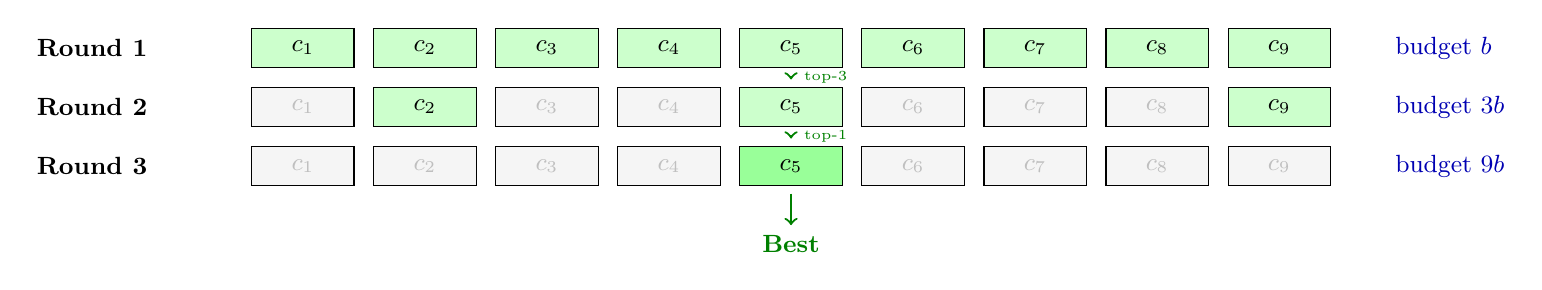
\begin{tikzpicture}[
          cell/.style={
            draw, minimum width=1.3cm, minimum height=0.5cm,
            font=\small, inner sep=2pt, anchor=center
          },
          active/.style={cell, fill=green!20},
          elim/.style={cell, fill=gray!8, text=gray!50},
          rndlabel/.style={font=\small\bfseries, anchor=east},
          budlabel/.style={font=\small, anchor=west, text=blue!70!black},
        ]
          \def\rowsep{0.75}

          % --- Round 1: 9 configs, budget b ---
          \node[rndlabel] at (-0.3, 0) {Round 1};
          \foreach \i in {1,...,9} {
            \node[active] at (\i*1.55, 0) {$c_{\i}$};
          }
          \node[budlabel] at (15.3, 0) {budget $b$};

          % Arrow round 1 -> 2
          \draw[->, thick, green!50!black] (5*1.55, -0.35) -- (5*1.55, -\rowsep+0.35)
            node[midway, right=1pt, font=\tiny] {top-3};

          % --- Round 2: 3 survivors, 6 eliminated ---
          \node[rndlabel] at (-0.3, -\rowsep) {Round 2};
          \foreach \i in {1,3,4,6,7,8} {
            \node[elim] at (\i*1.55, -\rowsep) {$c_{\i}$};
          }
          \foreach \i in {2, 5, 9} {
            \node[active] at (\i*1.55, -\rowsep) {$c_{\i}$};
          }
          \node[budlabel] at (15.3, -\rowsep) {budget $3b$};

          % Arrow round 2 -> 3
          \draw[->, thick, green!50!black] (5*1.55, -\rowsep-0.35) -- (5*1.55, -2*\rowsep+0.35)
            node[midway, right=1pt, font=\tiny] {top-1};

          % --- Round 3: 1 winner ---
          \node[rndlabel] at (-0.3, -2*\rowsep) {Round 3};
          \foreach \i in {1,2,3,4,6,7,8,9} {
            \node[elim] at (\i*1.55, -2*\rowsep) {$c_{\i}$};
          }
          \node[active, fill=green!40] at (5*1.55, -2*\rowsep) {$c_{5}$};
          \node[budlabel] at (15.3, -2*\rowsep) {budget $9b$};

          % Winner annotation
          \draw[->, thick, green!50!black] (5*1.55, -2*\rowsep-0.35) -- (5*1.55, -2*\rowsep-0.75)
            node[below, font=\small\bfseries, green!50!black] {Best};
        \end{tikzpicture}%
        }
      \end{center}
      \vspace{-0.3em}
      {\scriptsize Example: $n{=}9$, $\eta{=}3$. Each round keeps top $\nicefrac{1}{\eta}$ and multiplies budget by~$\eta$.}
    \end{column}
  \end{columns}
\end{frame}

% -----------------------------------------------------------------------
\begin{frame}{Hyperband}

  \textbf{Problem with SHA:} Must choose $n$ upfront: trade-off between coverage and early stopping aggressiveness.

  \vspace{0.3em}
  \textbf{Hyperband}~\cite{li2017hyperband} runs \emph{multiple independent SHA instances} (called \emph{brackets}) in parallel, each with a different $n$-vs-budget trade-off:

  \vspace{0.2em}
  \begin{columns}[T]
    \begin{column}{0.55\textwidth}
      \textbf{Setup:} Given total budget $B$ and $\eta$, create $s_{\max}{+}1$ brackets.
      Each bracket \emph{independently} samples its own fresh random configs:
      \begin{description}[leftmargin=0.5em]
        \item[Brk 0:] sample 81 configs, start at budget $b{=}1$
        \item[Brk 1:] sample 9 configs, start at budget $b{=}3$
        \item[Brk 2:] sample 6 configs, start at budget $b{=}9$
        \item[Brk 3:] sample 4 configs, start at budget $b{=}27$
      \end{description}
      \vspace{0.2em}
      \textbf{Within each bracket:} run SHA: evaluate, keep best $\nicefrac{1}{\eta}$, multiply budget by $\eta$, repeat.

      \vspace{0.2em}
      \textbf{Output:} Return the best config across all brackets.
    \end{column}
    \begin{column}{0.42\textwidth}
      \begin{center}
        \resizebox{\columnwidth}{!}{%
        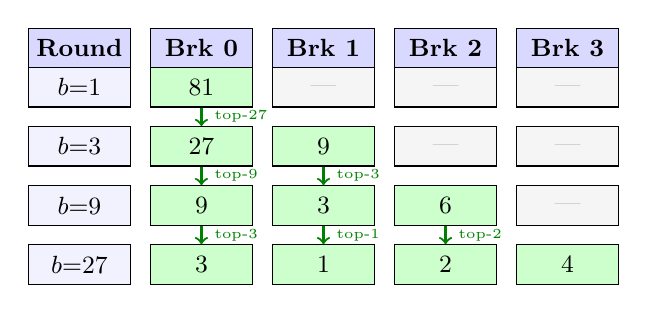
\begin{tikzpicture}[
          cell/.style={
            draw, minimum width=1.3cm, minimum height=0.5cm,
            font=\small, inner sep=2pt, anchor=center
          },
          header/.style={cell, fill=blue!15, font=\small\bfseries},
          active/.style={cell, fill=green!20},
          empty/.style={cell, fill=gray!8, text=gray!50},
        ]
          \def\colsep{1.55}
          \def\rowsep{0.75}

          % Column headers
          \node[header] at (0, 0.5) {Round};
          \node[header] at (1*\colsep, 0.5) {Brk 0};
          \node[header] at (2*\colsep, 0.5) {Brk 1};
          \node[header] at (3*\colsep, 0.5) {Brk 2};
          \node[header] at (4*\colsep, 0.5) {Brk 3};

          % Round column
          \node[cell, fill=blue!5] at (0, -0*\rowsep) {$b{=}1$};
          \node[cell, fill=blue!5] at (0, -1*\rowsep) {$b{=}3$};
          \node[cell, fill=blue!5] at (0, -2*\rowsep) {$b{=}9$};
          \node[cell, fill=blue!5] at (0, -3*\rowsep) {$b{=}27$};

          % Bracket 0
          \node[active] (b0r0) at (1*\colsep, -0*\rowsep) {81};
          \node[active] (b0r1) at (1*\colsep, -1*\rowsep) {27};
          \node[active] (b0r2) at (1*\colsep, -2*\rowsep) {9};
          \node[active] (b0r3) at (1*\colsep, -3*\rowsep) {3};

          % Bracket 1
          \node[empty] at (2*\colsep, -0*\rowsep) {---};
          \node[active] (b1r1) at (2*\colsep, -1*\rowsep) {9};
          \node[active] (b1r2) at (2*\colsep, -2*\rowsep) {3};
          \node[active] (b1r3) at (2*\colsep, -3*\rowsep) {1};

          % Bracket 2
          \node[empty] at (3*\colsep, -0*\rowsep) {---};
          \node[empty] at (3*\colsep, -1*\rowsep) {---};
          \node[active] (b2r2) at (3*\colsep, -2*\rowsep) {6};
          \node[active] (b2r3) at (3*\colsep, -3*\rowsep) {2};

          % Bracket 3
          \node[empty] at (4*\colsep, -0*\rowsep) {---};
          \node[empty] at (4*\colsep, -1*\rowsep) {---};
          \node[empty] at (4*\colsep, -2*\rowsep) {---};
          \node[active] (b3r3) at (4*\colsep, -3*\rowsep) {4};

          % Arrows within Bracket 0
          \draw[->, thick, green!50!black] (b0r0.south) -- (b0r1.north) node[midway, right=1pt, font=\tiny] {top-27};
          \draw[->, thick, green!50!black] (b0r1.south) -- (b0r2.north) node[midway, right=1pt, font=\tiny] {top-9};
          \draw[->, thick, green!50!black] (b0r2.south) -- (b0r3.north) node[midway, right=1pt, font=\tiny] {top-3};

          % Arrows within Bracket 1
          \draw[->, thick, green!50!black] (b1r1.south) -- (b1r2.north) node[midway, right=1pt, font=\tiny] {top-3};
          \draw[->, thick, green!50!black] (b1r2.south) -- (b1r3.north) node[midway, right=1pt, font=\tiny] {top-1};

          % Arrow within Bracket 2
          \draw[->, thick, green!50!black] (b2r2.south) -- (b2r3.north) node[midway, right=1pt, font=\tiny] {top-2};
        \end{tikzpicture}%
        }
      \end{center}
      \vspace{-0.2em}
      {\scriptsize Cells = \#configs at each budget level ($\eta{=}3$). Arrows: top-$\nicefrac{1}{\eta}$ advance to next round.}
    \end{column}
  \end{columns}

  \vspace{0.3em}
  Each bracket uses $\approx$ the same total compute. Provides $\approx \log(B_{\max})$ speedup over random search.

\end{frame}

% -----------------------------------------------------------------------
\begin{frame}{TPE: Tree-structured Parzen Estimator}

  \begin{columns}[T]
    \begin{column}{0.50\textwidth}
      TPE follows the idea of Bayesian optimization but takes a different approach~\cite{bergstra2011algorithms}.

      \vspace{0.2em}
      \textbf{KDE:} Given points $\{x_1, \ldots, x_n\}$, estimate a smooth density:
      $\hat{p}(x) = \frac{1}{n} \sum_{i} K_h(x - x_i)$

      \vspace{0.3em}
      \textbf{Core idea:} Split trials at threshold $y^*$ (e.g.\ top 20\%). Fit a KDE to each group:
      \[
        p(\vx \mid y) {=} \begin{cases}
          \ell(\vx) & y < y^* ~ \text{(good)} \\
          g(\vx)    & y \geq y^* ~ \text{(bad)}
        \end{cases}
      \]

      \vspace{0.2em}
      \textbf{Next config:} Sample from $\ell(\vx)$, pick the one maximizing $\ell(\vx) / g(\vx)$.
      \begin{itemize}
        \item High $\ell$: looks good. Low $g$: not bad.
        \item $\ell/g \propto$ Expected Improvement
      \end{itemize}

      \vspace{0.2em}
      {\small Each HP modelled independently $\Rightarrow$ scales to many dims. Default in Optuna~\cite{akiba2019optuna}.}

      \vspace{0.2em}
      {\small \textbf{Note:} TPE can be understood as Bayesian optimization where the density ratio $\ell/g$ plays the role of the acquisition function~\cite{snoek2012practical}.}
    \end{column}
    \begin{column}{0.47\textwidth}
      \begin{center}
        \resizebox{\columnwidth}{!}{%
        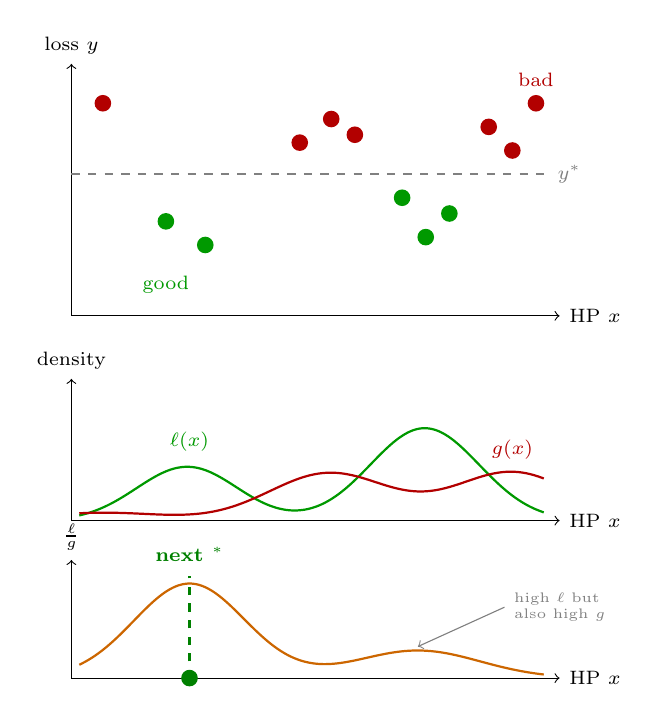
\begin{tikzpicture}
          % --- Top plot: observations split into good/bad ---
          \begin{scope}[shift={(0,0.6)}]
            \draw[->] (0,0) -- (6.2,0) node[right, font=\scriptsize] {HP $x$};
            \draw[->] (0,0) -- (0,3.2) node[above, font=\scriptsize] {loss $y$};

            % Threshold line
            \draw[dashed, gray, thick] (0, 1.8) -- (6, 1.8);
            \node[font=\scriptsize, gray, anchor=west] at (6.05, 1.8) {$y^*$};

            % Good trials: cluster A around x~1.5 (2 points), cluster B around x~4.5 (3 points)
            \fill[green!60!black] (1.2, 1.2) circle (3pt);
            \fill[green!60!black] (1.7, 0.9) circle (3pt);
            \fill[green!60!black] (4.2, 1.5) circle (3pt);
            \fill[green!60!black] (4.5, 1.0) circle (3pt);
            \fill[green!60!black] (4.8, 1.3) circle (3pt);

            % Bad trials: flanking cluster B on both sides (x~3-3.5 and x~5.3-5.8), plus one far left
            \fill[red!70!black] (0.4, 2.7) circle (3pt);
            \fill[red!70!black] (2.9, 2.2) circle (3pt);
            \fill[red!70!black] (3.3, 2.5) circle (3pt);
            \fill[red!70!black] (3.6, 2.3) circle (3pt);
            \fill[red!70!black] (5.3, 2.4) circle (3pt);
            \fill[red!70!black] (5.6, 2.1) circle (3pt);
            \fill[red!70!black] (5.9, 2.7) circle (3pt);

            \node[font=\scriptsize, green!60!black] at (1.2, 0.4) {good};
            \node[font=\scriptsize, red!70!black] at (5.9, 3.0) {bad};
          \end{scope}

          % --- Middle plot: two KDEs ---
          \begin{scope}[shift={(0,-2.0)}]
            \draw[->] (0,0) -- (6.2,0) node[right, font=\scriptsize] {HP $x$};
            \draw[->] (0,0) -- (0,1.8) node[above, font=\scriptsize] {density};

            % l(x) - two peaks: smaller at x~1.5, larger at x~4.5
            \draw[thick, green!60!black, domain=0.1:6, samples=100, smooth]
              plot (\x, {0.35*exp(-1.5*(\x-1.2)*(\x-1.2)) + 0.4*exp(-1.5*(\x-1.7)*(\x-1.7))
                + 0.4*exp(-1.2*(\x-4.2)*(\x-4.2)) + 0.5*exp(-1.2*(\x-4.5)*(\x-4.5))
                + 0.35*exp(-1.2*(\x-4.8)*(\x-4.8))});
            \node[font=\scriptsize, green!60!black, anchor=south] at (1.5, 0.75) {$\ell(x)$};

            % g(x) - flanking cluster B: peaks around x~3.2 and x~5.6
            \draw[thick, red!70!black, domain=0.1:6, samples=100, smooth]
              plot (\x, {0.1*exp(-0.8*(\x-0.4)*(\x-0.4))
                + 0.2*exp(-1.0*(\x-2.9)*(\x-2.9)) + 0.25*exp(-1.0*(\x-3.3)*(\x-3.3))
                + 0.2*exp(-1.0*(\x-3.6)*(\x-3.6))
                + 0.2*exp(-1.0*(\x-5.3)*(\x-5.3)) + 0.25*exp(-1.0*(\x-5.6)*(\x-5.6))
                + 0.2*exp(-1.0*(\x-5.9)*(\x-5.9))});
            \node[font=\scriptsize, red!70!black, anchor=south] at (5.6, 0.65) {$g(x)$};
          \end{scope}

          % --- Bottom plot: ratio l/g ---
          \begin{scope}[shift={(0,-4.0)}]
            \draw[->] (0,0) -- (6.2,0) node[right, font=\scriptsize] {HP $x$};
            \draw[->] (0,0) -- (0,1.5) node[above, font=\scriptsize] {$\frac{\ell}{g}$};

            % Ratio: high peak at x~1.5 (good, no bad), smaller peak at x~4.5 (good but also bad)
            \draw[thick, orange!80!black, domain=0.1:6, samples=100, smooth]
              plot (\x, {max(0.02, 1.2*exp(-1.0*(\x-1.5)*(\x-1.5))
                + 0.35*exp(-0.8*(\x-4.4)*(\x-4.4)))});

            % Next sample marker at x~1.5 (the better ratio)
            \draw[thick, green!50!black, dashed] (1.5, 0) -- (1.5, 1.3);
            \fill[green!50!black] (1.5, 0) circle (3pt);
            \node[font=\scriptsize\bfseries, green!50!black, anchor=south] at (1.5, 1.35) {next $\vx^*$};

            % Annotation for the smaller peak
            \draw[<-, gray, thin] (4.4, 0.4) -- (5.5, 0.9)
              node[right, font=\tiny, gray, align=left] {high $\ell$ but\\also high $g$};
          \end{scope}
        \end{tikzpicture}%
        }
      \end{center}
    \end{column}
  \end{columns}

\end{frame}

% -----------------------------------------------------------------------
\begin{frame}{BOHB: Bayesian Optimization and Hyperband}

  \textbf{Problem:} Hyperband explores broadly but samples configs \emph{randomly}. TPE samples intelligently but evaluates each config to completion (no early stopping).

  \vspace{0.3em}
  \textbf{BOHB}~\cite{falkner2018bohb} combines both: use TPE to \emph{sample} configs, Hyperband to \emph{schedule} them.

  \vspace{0.3em}
  \textbf{Algorithm:}
  \begin{enumerate}
    \item Run Hyperband's bracket structure (multiple SHA instances with different budgets)
    \item Instead of sampling configs uniformly at random, use a \textbf{TPE model} fitted on completed evaluations at the \emph{current budget level}
    \item As more configs finish, the TPE model improves $\Rightarrow$ later configs are better
  \end{enumerate}

  \vspace{0.3em}
  \textbf{Key design choices:}
  \begin{itemize}
    \item Fit TPE only on results from the \emph{same budget level} (short runs inform short-run sampling, long runs inform long-run sampling)
    \item Fall back to random sampling until enough observations exist (typically $\geq$\,10)
    \item Inherits Hyperband's parallelism: multiple brackets run concurrently
  \end{itemize}

  \vspace{0.3em}
  \textbf{Result:} Matches Hyperband's fast early progress \emph{and} TPE's late-stage refinement. Consistently among the best methods across benchmarks.

\end{frame}

% -----------------------------------------------------------------------
\begin{frame}{Comparing HPO Methods}

  When controlling for total compute budget, there is no single best method~\cite{falkner2018bohb}.

  \vspace{0.3em}
  \begin{center}
    \renewcommand{\arraystretch}{1.3}
    \resizebox{\textwidth}{!}{%
    \begin{tabular}{llll}
      \toprule
      \textbf{Method} & \textbf{Strengths} & \textbf{Weaknesses} & \textbf{Speedup vs.\ RS} \\
      \midrule
      Random search & Trivially parallel, strong baseline & No learning from past trials & $1\times$ (baseline) \\
      Hyperband / SHA & Fast with small budgets; explores broadly & Relies on cheap proxies being informative & $5$--$30\times$ \\
      TPE / Bayesian opt. & Exploits structure; best with few HPs & Sequential; slow start & $2$--$5\times$ \\
      BOHB & Informed sampling + early stopping & More complex to implement & $10$--$50\times$ \\
      \bottomrule
    \end{tabular}%
    }
  \end{center}
  {\scriptsize Speedups from \cite{li2017hyperband} and \cite{falkner2018bohb}, measured as wall-clock time to reach target validation error on neural network benchmarks.}

  \vspace{0.3em}
  \textbf{Key findings:}
  \begin{itemize}
    \item \textbf{Small compute budget:} Hyperband wins: aggressive early stopping explores more configs
    \item \textbf{Large compute budget:} Bayesian methods (TPE) win: learned surrogate model pays off
    \item \textbf{General purpose:} BOHB (Hyperband + TPE) rarely loses badly to any single method
    \item \textbf{Random search} is competitive in high dimensions and embarrassingly parallel settings
  \end{itemize}

\end{frame}

% -----------------------------------------------------------------------
\subsection{Learning Rate Schedules}

% -----------------------------------------------------------------------
\begin{frame}{LR Range Test}

  The learning rate $\eta$ controls the step size of gradient updates.
  Too high $\Rightarrow$ divergence. Too low $\Rightarrow$ slow convergence / poor optima.

  \vspace{0.4em}
  \begin{columns}[T]
    \begin{column}{0.50\textwidth}
      \textbf{LR Range Test}~\cite{smith2017cyclical}: a quick diagnostic before a full training run.
      \begin{itemize}
        \item Increase $\eta$ exponentially from very small to very large over one epoch
        \item Plot loss vs.\ $\eta$; the optimal range is where loss decreases fastest (steepest descent), \emph{not} the minimum
      \end{itemize}

      \medskip
      \textbf{Reading the curve:}
      \begin{itemize}
        \item If loss spikes early: reduce LR or increase warmup
        \item If loss plateaus: try $2\text{--}3\times$ higher LR
      \end{itemize}
    \end{column}
    \begin{column}{0.48\textwidth}
      \begin{center}
      \begin{tikzpicture}[scale=0.85]
        \draw[->, thick] (0,0) -- (5,0) node[below, font=\scriptsize] {$\log \eta$};
        \draw[->, thick] (0,0) -- (0,3.5) node[above, font=\scriptsize] {loss};
        % Loss curve: flat, then decrease, then increase
        \draw[slide_blue!80!black, very thick] plot[smooth, tension=0.6] coordinates
          {(0.2,2.8) (1.0,2.7) (1.8,2.3) (2.5,1.5) (3.2,1.2) (3.8,1.8) (4.5,3.2)};
        % Good region
        \draw[green!60!black, very thick, <->] (1.5, 0.3) -- (3.3, 0.3);
        \node[green!60!black, font=\scriptsize, above] at (2.4, 0.3) {good range};
        % Annotation
        \draw[->, gray, thin] (4.2, 2.8) -- (4.5, 3.1);
        \node[gray, font=\tiny, left] at (4.2, 2.7) {diverges};
      \end{tikzpicture}
      \end{center}
      {\small Sweep $\eta$ exponentially over one epoch. Pick the range where loss drops fastest, not the minimum.}
    \end{column}
  \end{columns}
\end{frame}

% -----------------------------------------------------------------------
\begin{frame}{Learning Rate Warmup}

  \textbf{Problem:} Adam's moving-average estimates $m_t, v_t$ are initialized to zero.
  Early in training they are heavily biased, so the effective step sizes $m_t / \sqrt{v_t}$ can be unreliable and cause divergent updates.

  \vspace{0.4em}
  \textbf{Solution:} Start with $\eta \approx 0$ and linearly increase to the target $\eta_{\max}$ over a \emph{warmup period}, giving the moment estimates time to stabilize~\cite{goyal2017accurate}.

  \[
    \eta_t = \begin{cases}
      \eta_{\max} \cdot \frac{t}{T_{\text{warmup}}} & \text{if } t \leq T_{\text{warmup}} \\
      \text{schedule}(\eta_{\max}, t) & \text{otherwise}
    \end{cases}
  \]

  \vspace{0.3em}
  \textbf{Typical warmup durations:}
  \begin{itemize}
    \item GPT-3: 375M tokens ($\approx$ 0.1\% of training)~\cite{brown2020gpt3}
    \item LLaMA: 2000 steps (of $\sim$1.0--1.4T tokens total)~\cite{touvron2023llama}
    \item Chinchilla: 5B tokens (of 1.4T tokens total)~\cite{hoffmann2022chinchilla}
    \item Rule of thumb: $\sim$0.1--1\% of total training steps
  \end{itemize}

  \vspace{0.3em}
  \textbf{Why it works:}
  \begin{itemize}
    \item Gives Adam's moment estimates ($m_t$, $v_t$) enough samples to become reliable
    \item Also helps with large early gradients (complementary to gradient clipping)
    \item Especially important with large batch sizes: linear scaling rule $\Rightarrow$ larger LR $\Rightarrow$ unreliable early steps are amplified
  \end{itemize}
\end{frame}

% -----------------------------------------------------------------------
\begin{frame}{Learning Rate Schedule and Decay}

  After warmup, the learning rate is \emph{decayed} toward a small final value.
  Decaying lets the optimizer settle into sharper minima as training progresses.

  \vspace{0.4em}
  \textbf{Common LR schedules for LLM pretraining:}

  \vspace{0.2em}
  \begin{center}
    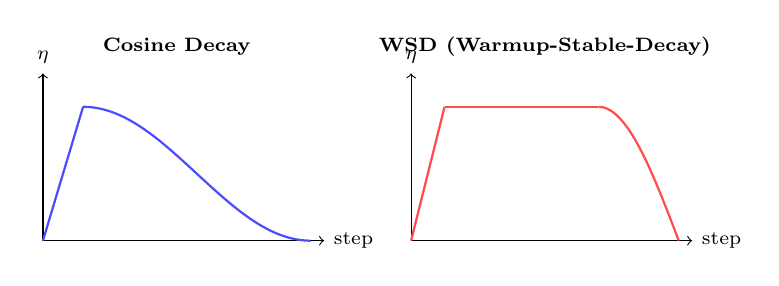
\begin{tikzpicture}[scale=0.85]
      % Cosine schedule
      \begin{scope}[shift={(0,0)}]
        \draw[->] (0,0) -- (4.2,0) node[right, font=\scriptsize] {step};
        \draw[->] (0,0) -- (0,2.5) node[above, font=\scriptsize] {$\eta$};
        \node[font=\scriptsize\bfseries] at (2,2.9) {Cosine Decay};
        % warmup
        \draw[thick, blue!70] (0,0) -- (0.6,2);
        % cosine decay
        \draw[thick, blue!70, domain=0.6:4, samples=100] plot (\x, {1.0 + 1.0*cos((\x-0.6)/(4-0.6)*180)});
      \end{scope}
      % WSD schedule
      \begin{scope}[shift={(5.5,0)}]
        \draw[->] (0,0) -- (4.2,0) node[right, font=\scriptsize] {step};
        \draw[->] (0,0) -- (0,2.5) node[above, font=\scriptsize] {$\eta$};
        \node[font=\scriptsize\bfseries] at (2,2.9) {WSD (Warmup-Stable-Decay)};
        % warmup
        \draw[thick, red!70] (0,0) -- (0.5,2);
        % stable
        \draw[thick, red!70] (0.5,2) -- (2.8,2);
        % decay
        \draw[thick, red!70, domain=2.8:4, samples=50] plot (\x, {2.0*cos((\x-2.8)/(4-2.8)*90)});
      \end{scope}
    \end{tikzpicture}
  \end{center}

  \vspace{0.2em}
  \begin{description}[labelwidth=\widthof{\bfseries Cosine decay~~}, leftmargin=!]
    \item[Cosine decay]~\cite{loshchilov2017sgdr}: Smoothly anneals $\eta$ from $\eta_{\max}$ to, e.g., $0.1\,\eta_{\max}$ following a half cosine. Standard for GPT-3, LLaMA, Chinchilla. Requires fixing the total step count in advance.
    \item[WSD] (Warmup-Stable-Decay)~\cite{hu2024minicpm}: Hold $\eta$ constant, then decay only over the final $\sim$10\% of steps. Introduced by MiniCPM; allows extending training without restarting, since the stable phase has no preset endpoint.
  \end{description}
\end{frame}

% -----------------------------------------------------------------------
\begin{frame}{Choosing a Good Learning Rate}

  \begin{columns}[T]
    \begin{column}{0.50\textwidth}
      \textbf{Safe LR regimes by task:}
      \begin{description}[labelwidth=\widthof{\bfseries From scratch~~}, leftmargin=!]
        \item[From scratch] $10^{-4}$--$10^{-3}$ (Adam/AdamW). Larger models $\Rightarrow$ lower end. Use LR range test or $\mu$P to narrow down.
        \item[Fine-tune] $10^{-5}$--$5 \times 10^{-5}$ (full fine-tuning). $10\text{--}50\times$ smaller than pretraining LR to avoid catastrophic forgetting.
        \item[LoRA/PEFT] $10^{-4}$--$3 \times 10^{-4}$. Adapters have few parameters $\Rightarrow$ can tolerate higher LR than full fine-tuning.
        \item[SGD (vision)] $10^{-2}$--$10^{-1}$. SGD needs $\sim$$100\times$ higher LR than Adam since it lacks adaptive scaling.
      \end{description}

      \medskip
      \textbf{Muon}~\cite{jordan2024muon} hyperparameters:
      \begin{itemize}
        \item Hidden 2D weights: $\eta \approx 10^{-2}$--$5{\times}10^{-2}$, far larger than Adam
        \item Embeddings, head, and scalar (norm/bias) params stay on Adam at $\sim$$10^{-3}$
        \item $\eta$ transfers well across width and depth, so little retuning is needed at scale
      \end{itemize}
    \end{column}
    \begin{column}{0.48\textwidth}
      \textbf{LR vs.\ model size:} bigger models want smaller LR ($\eta$ roughly $\propto 1/\sqrt{\text{width}}$).
      \[
        \underbrace{10^{-2}}_{\lesssim 10\text{M}} \to
        \underbrace{6{\times}10^{-4}}_{100\text{M}} \to
        \underbrace{3{\times}10^{-4}}_{1\text{B}} \to
        \underbrace{6{\times}10^{-5}}_{\gtrsim 100\text{B}}
      \]
      {\scriptsize Adam, from scratch (GPT-2/GPT-3 scale). $\mu$P makes the optimal LR roughly width-invariant.}

      \medskip
      \textbf{Rules of thumb:}
      \begin{itemize}
        \item Narrow down the starting LR with an LR range test or $\mu$P before committing to a full run
        \item If loss spikes early: reduce LR or increase warmup
        \item If loss plateaus: try $2\text{--}3\times$ higher LR
        \item When scaling batch size $B \to kB$: scale $\eta \to k\eta$ (linear) or $\eta \to \sqrt{k}\,\eta$ (square root)
      \end{itemize}
    \end{column}
  \end{columns}
\end{frame}

% -----------------------------------------------------------------------
\begin{frame}{Training with a Pretrained Backbone}

  A pretrained \emph{backbone} feeds a small, randomly initialized task-specific \emph{head}.

  \vspace{0.3em}
  \begin{columns}[T]
    \begin{column}{0.54\textwidth}
      \textbf{Full fine-tuning:}
      \begin{itemize}
        \item Warm up the head first (freeze backbone briefly) so its random gradients do not corrupt good features
        \item Backbone LR $10$--$100\times$ smaller than head LR: e.g.\ head $\sim 10^{-3}$, backbone $\sim 10^{-5}$--$10^{-4}$
      \end{itemize}

      \vspace{0.3em}
      \textbf{Layer-wise LR decay (LLRD):} generalize this, decaying the LR \emph{geometrically} from head down to embeddings:
      \[
        \eta_\ell = \eta_{\text{top}} \cdot \xi^{\,L - \ell}, \qquad \xi \approx 0.65\text{--}0.9
      \]
      \begin{itemize}
        \item Top layers adapt fast; bottom layers barely move, preserving general features and reducing catastrophic forgetting
      \end{itemize}

      \vspace{0.2em}
      {\scriptsize Discriminative fine-tuning, from ULMFiT~\cite{howard2018ulmfit}; standard for BERT/ELECTRA~\cite{clark2020electra} and ViT.}
    \end{column}
    \begin{column}{0.42\textwidth}
      \begin{center}
      \begin{tikzpicture}[scale=0.85,
        blk/.style={draw, rounded corners=2pt, minimum width=2.2cm, minimum height=0.5cm, font=\scriptsize}]
        % backbone layers (light to dark) + head
        \node[blk, fill=slide_blue!20] (l0) at (0,0)   {embeddings};
        \node[blk, fill=slide_blue!35] (l1) at (0,0.8) {layer 1};
        \node[blk, fill=slide_blue!50] (l2) at (0,1.6) {layer 2};
        \node[blk, fill=slide_blue!65] (l3) at (0,2.4) {layer 3};
        \node[blk, fill=orange!35]     (hd) at (0,3.4) {head};
        % LR labels on the right
        \node[font=\scriptsize, anchor=west] at (1.25, 0)   {$\eta\,\xi^{4}$};
        \node[font=\scriptsize, anchor=west] at (1.25, 0.8) {$\eta\,\xi^{3}$};
        \node[font=\scriptsize, anchor=west] at (1.25, 1.6) {$\eta\,\xi^{2}$};
        \node[font=\scriptsize, anchor=west] at (1.25, 2.4) {$\eta\,\xi^{1}$};
        \node[font=\scriptsize, anchor=west] at (1.25, 3.4) {$\eta$};
        % braces on the left (point left: draw bottom -> top)
        \draw[decorate, decoration={brace, amplitude=4pt}, slide_blue!80!black]
          (-1.25, -0.25) -- (-1.25, 2.65)
          node[midway, left=4pt, font=\scriptsize, align=right, text=slide_blue!80!black]
          {backbone\\(pretrained)};
        \draw[decorate, decoration={brace, amplitude=4pt}, orange!80!black]
          (-1.25, 3.15) -- (-1.25, 3.65)
          node[midway, left=4pt, font=\scriptsize, align=right, text=orange!80!black]
          {head\\(random)};
      \end{tikzpicture}
      \end{center}
    \end{column}
  \end{columns}
\end{frame}

% -----------------------------------------------------------------------
\subsection{Batch Size Selection}

% -----------------------------------------------------------------------
\begin{frame}{Critical Batch Size}

  \textbf{Why maximize batch size?} Larger $B$ means fewer gradient steps per epoch $\Rightarrow$ fewer synchronization rounds in distributed training, better GPU utilization, and faster wall-clock time. But there is a limit:

  \medskip
  \begin{columns}[T]
    \begin{column}{0.52\textwidth}
      \textbf{Critical batch size}~\cite{mccandlish2018empirical}:
      \begin{itemize}
        \item Below $B_{\text{crit}}$: doubling $B$ halves training time (perfect scaling)
        \item Above $B_{\text{crit}}$: diminishing returns, extra samples are mostly wasted
        \item $B_{\text{crit}} \propto 1/L$: smaller loss $\Rightarrow$ larger $B_{\text{crit}}$, so it \emph{grows} during training
      \end{itemize}

      \medskip
      Batch size is thus mostly a \emph{systems} knob: within the efficient regime it trades wall-clock time against gradient noise, with accuracy roughly unchanged once the LR is adjusted.
    \end{column}
    \begin{column}{0.46\textwidth}
      \centering
      \begin{tikzpicture}[scale=0.85]
        % Axes
        \draw[->, thick] (0,0) -- (5.2,0) node[below] {\small batch size $B$};
        \draw[->, thick] (0,0) -- (0,4.2) node[above, font=\small] {steps $S$};

        % Steps to converge: S ~ 1/B for B < Bcrit, then flattens (S ~ S_min + Bcrit/B models this)
        \draw[slide_blue!80!black, very thick]
          plot[smooth, domain=0.3:5, samples=50]
          (\x, {0.6 + 3.0 * 0.3 / \x});

        % B_crit dashed line
        \draw[dashed, thick, gray] (1.4, 0) -- (1.4, 3.8);
        \node[below, font=\small] at (1.4, 0) {$B_{\text{crit}}$};

        % Region labels
        \node[font=\scriptsize, text=green!50!black, align=center] at (0.7, 3.6) {perfect\\[-2pt]scaling};
        \node[font=\scriptsize, text=red!60!black, align=center] at (3.5, 3.0) {diminishing\\[-2pt]returns};
      \end{tikzpicture}
    \end{column}
  \end{columns}

  \medskip
  \textbf{Typical scales} ($B_{\text{crit}}$ grows with task difficulty and lower loss; practical $B$ is set near it):
  \begin{description}[labelwidth=\widthof{\bfseries Vision~~}, leftmargin=!]
    \item[Vision] small: MNIST $\sim$ tens, CIFAR/ImageNet $\sim 10^3$--$10^4$ images (ViT-L: 4096, CLIP: 32k pairs)
    \item[LLM] large: $\sim 10^5$--$10^7$ tokens, rising through training (GPT-3: 3.2M, LLaMA-2: 4M, DeepSeek-V3: 15.6M)
    \item[RL] highly variable: $\sim 10^4$ (simple control) up to $\sim 10^7$ (Dota-scale) state-action pairs
  \end{description}
\end{frame}

% -----------------------------------------------------------------------
\begin{frame}{How to Choose the Batch Size}

  Given the critical batch size, choosing $B$ is a practical recipe:

  \vspace{0.4em}
  \textbf{General procedure:}
  \begin{enumerate}
    \item \textbf{Start from hardware:} pick the largest per-device batch that fits in memory; multiply by the number of devices and gradient-accumulation steps to get the global batch.
    \item \textbf{Stay below $B_{\text{crit}}$:} going past it buys little speedup while burning compute.
    \item \textbf{Ramp up over training:} since $B_{\text{crit}}$ grows as the loss falls, start small and increase $B$ to stay in the efficient regime.
  \end{enumerate}

  \vspace{0.3em}
  \textbf{Rules of thumb:}
  \begin{itemize}
    \item Prefer powers of two (and multiples of 8/64) for good GPU/tensor-core utilization
    \item If you cannot fit the target batch, use gradient accumulation to emulate it
    \item Whenever you change $B$, the learning rate must be retuned (see next slides)
  \end{itemize}

\end{frame}

% -----------------------------------------------------------------------
\begin{frame}{Batch Size and the Linear Scaling Rule}

  The mini-batch gradient \emph{averages} over $B$ random samples:
  \[
    \hat{g}_B = \frac{1}{B} \sum_{i=1}^{B} \nabla L_i(\vw) \qquad \Rightarrow \qquad \vw_{t+1} = \vw_t - \eta\, \hat{g}_B
  \]

  \vspace{0.2em}
  \textbf{Linear scaling rule}~\cite{goyal2017accurate}: With $k\times$ larger batch we take $k\times$ fewer steps per epoch. To cover the same distance in weight space, scale $\eta \to k\eta$:

  \medskip
  \begin{center}
  \begin{minipage}[c]{0.42\textwidth}
  \begin{tcolorbox}[colback=slide_blue!30, colframe=slide_blue!80, boxrule=0.6pt, arc=3pt, left=6pt, right=6pt, top=4pt, bottom=4pt]
    \centering
    {\small\textbf{1 step, batch $kB$, rate $k\eta$}}\\[4pt]
    $\vw - k\eta\, \hat{g}_{kB}$
  \end{tcolorbox}
  \end{minipage}%
  \hfill
  \begin{minipage}[c]{0.06\textwidth}
    \centering $\approx$
  \end{minipage}%
  \hfill
  \begin{minipage}[c]{0.42\textwidth}
  \begin{tcolorbox}[colback=slide_beige!30, colframe=slide_beige!80, boxrule=0.6pt, arc=3pt, left=6pt, right=6pt, top=4pt, bottom=4pt]
    \centering
    {\small\textbf{$k$ steps, batch $B$, rate $\eta$}}\\[4pt]
    $\vw - \eta \displaystyle\sum_{j=1}^{k} \hat{g}_{B}^{(j)}$
  \end{tcolorbox}
  \end{minipage}
  \end{center}
  Both sides have the same \emph{expected} update: $\mathbb{E}[\hat{g}_{kB}] = \mathbb{E}[\hat{g}_B]$ because both are sample means of i.i.d.\ draws (batch size only affects variance, not expectation).

  \vspace{0.3em}
  \textbf{Limitations:}
  \begin{itemize}
    \item Assumes $\text{Var}[\hat{g}]$ is small enough that linear approximation holds, but breaks for very large $B$
    \item Derived for plain SGD; adaptive/normalized optimizers (AdamW, Muon) prefer square-root scaling instead (next slide)
    \item Requires LR warmup to work at large batch sizes
  \end{itemize}

\end{frame}

% -----------------------------------------------------------------------
\begin{frame}{Square Root Learning Rate Scaling}

  \textbf{Alternative:} Scale $\eta \to \sqrt{k}\,\eta$ when $B \to kB$~\cite{hoffer2017train}.

  \vspace{0.3em}
  \textbf{Motivation from gradient noise:}
  \begin{itemize}
    \item The gradient estimate has variance $\text{Var}[\hat{g}_B] = \sigma^2 / B$, so its std scales as $1/\sqrt{B}$
    \item One SGD step moves weights by $\Delta \vw = -\eta\, \hat{g}_B = -\eta\,(g + \varepsilon/\sqrt{B})$
    \item Scaling $\eta \to \sqrt{k}\,\eta$ with $B \to kB$ keeps the \emph{noise contribution} $\eta \cdot \sigma / \sqrt{B}$ constant
    \item Linear scaling ($\eta \to k\eta$) would amplify noise by $\sqrt{k}$
  \end{itemize}

  \vspace{0.3em}
  \textbf{Linear vs.\ square root scaling:}
  \begin{description}[labelwidth=\widthof{\bfseries Square root~~}, leftmargin=!]
    \item[Linear] Preserves expected update magnitude. Works well for moderate $k$ ($\leq 8$--$16$) with LR warmup. Default for plain SGD.
    \item[Square root] Preserves signal-to-noise ratio. More robust for very large $B$ (above $B_\text{crit}$) where linear scaling causes instability.
  \end{description}

  \vspace{0.3em}
  \textbf{Which rule for AdamW / Muon?} Both normalize the update, so the SGD linear rule does \emph{not} carry over: the analysis of the underlying SDEs shows adaptive optimizers should use the \emph{square-root} rule $\eta \to \sqrt{k}\,\eta$~\cite{malladi2022sde}.
  \begin{itemize}
    \item \textbf{AdamW:} division by $\sqrt{\hat{\vv}_t}$ already rescales the step, so $\eta \to \sqrt{k}\,\eta$ tracks the optimal LR; linear scaling overshoots at large $B$.
    \item \textbf{Muon:} updates are orthogonalized to $\approx$ unit scale, so they are even \emph{less} sensitive to $B$; use $\sqrt{k}$ as a starting point and retune mildly.
  \end{itemize}
  In practice the optimal exponent $\alpha$ in $\eta \to k^\alpha \eta$ lands between $0.5$ and $1.0$, depending on optimizer, model, and training stage.

\end{frame}

% -----------------------------------------------------------------------
\begin{frame}{Gradient Noise Scale and Batch Size Ramp-Up}

  \begin{columns}[T]
    \begin{column}{0.50\textwidth}
      \textbf{Gradient noise scale}~\cite{mccandlish2018empirical}:
      \begin{align*}
        G &= \mathbb{E}[\nabla L_i] \\
        \Sigma &= \text{Cov}(\nabla L_i) = \mathbb{E}[(\nabla L_i - G)(\nabla L_i - G)^\top] \\
        \mathcal{B}_{\text{noise}} &= \frac{\text{tr}(\Sigma)}{|G|^2}
      \end{align*}
      The mini-batch gradient has variance $\text{Var}[\hat{g}_B] = \Sigma / B$, so the noise-to-signal ratio of a step is:
      \[
        \frac{\text{tr}(\Sigma / B)}{|G|^2} = \frac{\mathcal{B}_{\text{noise}}}{B}
      \]
      \begin{itemize}
        \item $B \ll \mathcal{B}_{\text{noise}}$: ratio $\gg 1$, step is mostly noise $\Rightarrow$ but cheap, so efficient
        \item $B \approx \mathcal{B}_{\text{noise}}$: ratio $\approx 1$, noise $\approx$ signal $\Rightarrow$ sweet spot
        \item $B \gg \mathcal{B}_{\text{noise}}$: ratio $\ll 1$, very accurate but extra samples wasted
      \end{itemize}
    \end{column}
    \begin{column}{0.48\textwidth}
      \textbf{Batch size ramp-up:}

      Since $B_{\text{crit}} \propto 1/L$, it grows during training as loss decreases. Ramp up $B$ to stay in the efficient regime:

      \medskip
      \begin{algorithm}[H]
        \small
        \caption{Batch Size Schedule}
        \KwInput{$B_{\min}$, $B_{\max}$, ramp tokens $T_{\text{ramp}}$}
        $B \gets B_{\min}$\;
        \For{each training step $t$}{
          \uIf{tokens seen $< T_{\text{ramp}}$}{
            $B \gets B_{\min} + (B_{\max} - B_{\min}) \cdot \frac{\text{tokens seen}}{T_{\text{ramp}}}$\;
          }
          \Else{$B \gets B_{\max}$\;}
          Train one step with batch size $B$\;
        }
      \end{algorithm}

      \medskip
      {\small GPT-3: 32k $\to$ 3.2M tokens over first 4--12B tokens~\cite{brown2020gpt3}}
    \end{column}
  \end{columns}

  \vspace{0.2em}
  {\small
  \textbf{Finding $B_{\text{crit}} \approx \mathcal{B}_{\text{noise}}$ in practice:}
  \begin{itemize}
    \item \emph{Noise-scale estimate} (cheap): measure the squared gradient norm at a small and a large (micro)batch; their difference gives an unbiased estimate of $\text{tr}(\Sigma)$ and $|G|^2$, hence $\mathcal{B}_{\text{noise}}$. Re-measure periodically: it rises during training.
    \item \emph{Empirical sweep}: run short trainings at several $B$, plot steps-to-target-loss vs.\ $B$; the knee of the curve is $B_{\text{crit}}$.
  \end{itemize}}
\end{frame}

% -----------------------------------------------------------------------
\subsection{Other Hyperparameters}

% -----------------------------------------------------------------------
\begin{frame}{Weight Decay}

  \textbf{Weight decay} shrinks weights toward zero every step, penalizing large parameter norms. It regularizes and, in modern LLM training, also controls the effective learning-rate scale.

  \vspace{0.3em}
  \begin{columns}[T]
    \begin{column}{0.52\textwidth}
      \textbf{$L_2$ regularization vs.\ decoupled decay}~\cite{loshchilov2019adamw}:
      \begin{itemize}
        \item $L_2$: add $\tfrac{\lambda}{2}\|\vw\|^2$ to the loss $\Rightarrow$ gradient $+\lambda\vw$. In Adam this term is \emph{also} divided by $\sqrt{\hat{\vv}_t}$, so large-gradient weights get decayed \emph{less}.
        \item \textbf{AdamW} decouples decay from the gradient: apply it directly to the weights,
        \[
          \vw_{t+1} = \vw_t - \eta\Big(\tfrac{\hat{\vm}_t}{\sqrt{\hat{\vv}_t}+\epsilon} + \lambda\,\vw_t\Big)
        \]
        \item Decoupling makes the optimal $\lambda$ far more stable across LR and architecture.
      \end{itemize}
    \end{column}
    \begin{column}{0.44\textwidth}
      \textbf{Practice:}
      \begin{itemize}
        \item Typical $\lambda = 0.1$ for LLM pretraining; $0.01$--$0.05$ common in vision
        \item \textbf{Exclude} biases, LayerNorm/RMSNorm scales, and embeddings from decay
        \item Interacts with LR and batch size: what matters is the \emph{AdamW timescale} $\tau = B/(\eta\lambda D)$~\cite{bernstein2025powerlines}
        \item Too high $\Rightarrow$ underfitting; too low $\Rightarrow$ weights grow, loss can destabilize late in training
      \end{itemize}
    \end{column}
  \end{columns}
\end{frame}

% -----------------------------------------------------------------------
\begin{frame}{Adam Parameters: $\beta_1$, $\beta_2$, $\epsilon$}

  Adam/AdamW~\cite{kingma2015adam} maintain exponential moving averages of the gradient ($\vm_t$) and its square ($\vv_t$):
  \[
    \vm_t = \beta_1 \vm_{t-1} + (1{-}\beta_1)\vg_t, \qquad
    \vv_t = \beta_2 \vv_{t-1} + (1{-}\beta_2)\vg_t^2, \qquad
    \Delta\vw \propto \frac{\hat{\vm}_t}{\sqrt{\hat{\vv}_t}+\epsilon}
  \]

  \vspace{0.2em}
  \begin{description}[labelwidth=\widthof{\bfseries $\beta_2$ (2nd mom.)~~}, leftmargin=!]
    \item[$\beta_1$ (momentum)] Averages the gradient direction. Default $0.9$ ($\approx$ average over the last $\tfrac{1}{1-\beta_1}{=}10$ steps). Higher smooths more but reacts slower.
    \item[$\beta_2$ (2nd mom.)] Averages the squared gradient for per-coordinate scaling. LLMs use $0.95$ (window $\sim$20) rather than the classic $0.999$ (window $\sim$1000): shorter memory adapts faster to the noisy, non-stationary gradients of large-batch training and reduces loss spikes.
    \item[$\epsilon$] Numerical floor preventing division by zero. Default $10^{-8}$; some large-scale runs use $10^{-6}$--$10^{-5}$ for stability in low precision (BF16).
  \end{description}

  \vspace{0.2em}
  \textbf{Bias correction:} $\hat{\vm}_t = \vm_t/(1{-}\beta_1^t)$, $\hat{\vv}_t = \vv_t/(1{-}\beta_2^t)$ compensates for the zero initialization; without it early steps are strongly damped (a key motivation for LR warmup).
\end{frame}

% -----------------------------------------------------------------------
\begin{frame}{Gradient Clipping \& Other Regularizers}

  \begin{columns}[T]
    \begin{column}{0.52\textwidth}
      \textbf{Gradient clipping}~\cite{pascanu2013difficulty}: cap the \emph{global} norm of the gradient to avoid destructive updates from occasional huge gradients (loss spikes, bad batches):
      \[
        \vg \leftarrow \vg \cdot \min\!\Big(1,\ \frac{c}{\|\vg\|_2}\Big)
      \]
      \begin{itemize}
        \item Clip by \emph{global} norm over all parameters, not per-tensor
        \item Near-universal threshold $c = 1.0$ in LLM training
        \item Monitor the clip rate: frequent clipping late in training signals instability (lower LR or inspect data)
      \end{itemize}
    \end{column}
    \begin{column}{0.44\textwidth}
      \textbf{Dropout:} randomly zeroes activations with prob.\ $p$. Standard in vision/BERT ($p\approx0.1$), but usually \emph{disabled} for LLM pretraining (single epoch, data is the regularizer); often reintroduced for fine-tuning.

      \vspace{0.3em}
      \textbf{Label smoothing:} soften one-hot targets by $\varepsilon$ ($\approx 0.1$). Common in vision/translation; rare in LLM pretraining.

      \vspace{0.3em}
      \textbf{$z$-loss:} small penalty $\alpha\,(\log Z)^2$ on the softmax normalizer to keep logits bounded; stabilizes large-scale training (PaLM, DeepSeek).
    \end{column}
  \end{columns}

  \vspace{0.3em}
  {\small \textbf{Rule of thumb:} for LLM pretraining, grad clip $1.0$ on, dropout/label smoothing off; add them back when fine-tuning on smaller datasets where overfitting is the risk.}
\end{frame}

% -----------------------------------------------------------------------
\subsection{Scaling Laws}

% -----------------------------------------------------------------------
\begin{frame}{Neural Scaling Laws~\cite{kaplan2020scaling}}

  \textbf{Key discovery:} LLM test loss follows \emph{power laws} in model size $N$ (non-embedding params), dataset size $D$ (tokens), and compute $C$ (FLOPs):
  \[
    L(N) = \left(\frac{N_c}{N}\right)^{\!\alpha_N}\!,\quad
    L(D) = \left(\frac{D_c}{D}\right)^{\!\alpha_D}\!,\quad
    L(C) = \left(\frac{C_c}{C}\right)^{\!\alpha_C}
  \]

  \begin{center}
  \begin{tikzpicture}[scale=0.75]
    % --- L(N) plot ---
    \begin{scope}[shift={(0,0)}]
      \draw[->, thick] (0,0) -- (4.5,0) node[below, font=\scriptsize] {$\log N$};
      \draw[->, thick] (0,0) -- (0,3.5) node[above, font=\scriptsize] {$L$};
      \node[font=\scriptsize\bfseries] at (2.2, 3.8) {$L(N)$};
      % Power law: L = (Nc/N)^0.076, on log scale looks linear
      % Plot from N=10^7 to 10^12, L from ~3.8 to ~1.6
      \draw[slide_blue!80!black, very thick] plot[smooth, domain=0.2:4.2, samples=30]
        (\x, {3.2 - 0.55*\x});
      % Data points (Cerebras-GPT style)
      \foreach \x/\y in {0.4/3.0, 1.0/2.7, 1.6/2.4, 2.2/2.1, 2.8/1.8, 3.4/1.5} {
        \fill[slide_blue!80!black] (\x, \y) circle (2pt);
      }
      % Axis ticks
      \node[below, font=\tiny] at (0.4,0) {$10^7$};
      \node[below, font=\tiny] at (2.2,0) {$10^9$};
      \node[below, font=\tiny] at (4.0,0) {$10^{11}$};
    \end{scope}
    % --- L(D) plot ---
    \begin{scope}[shift={(5.5,0)}]
      \draw[->, thick] (0,0) -- (4.5,0) node[below, font=\scriptsize] {$\log D$};
      \draw[->, thick] (0,0) -- (0,3.5) node[above, font=\scriptsize] {$L$};
      \node[font=\scriptsize\bfseries] at (2.2, 3.8) {$L(D)$};
      \draw[red!70!black, very thick] plot[smooth, domain=0.2:4.2, samples=30]
        (\x, {3.0 - 0.5*\x});
      \foreach \x/\y in {0.5/2.8, 1.2/2.4, 1.9/2.1, 2.6/1.7, 3.3/1.4, 4.0/1.1} {
        \fill[red!70!black] (\x, \y) circle (2pt);
      }
      \node[below, font=\tiny] at (0.5,0) {$10^8$};
      \node[below, font=\tiny] at (2.2,0) {$10^{10}$};
      \node[below, font=\tiny] at (4.0,0) {$10^{12}$};
    \end{scope}
    % --- L(C) plot ---
    \begin{scope}[shift={(11,0)}]
      \draw[->, thick] (0,0) -- (4.5,0) node[below, font=\scriptsize] {$\log C$};
      \draw[->, thick] (0,0) -- (0,3.5) node[above, font=\scriptsize] {$L$};
      \node[font=\scriptsize\bfseries] at (2.2, 3.8) {$L(C)$};
      \draw[green!50!black, very thick] plot[smooth, domain=0.2:4.2, samples=30]
        (\x, {3.1 - 0.52*\x});
      \foreach \x/\y in {0.4/2.9, 1.1/2.5, 1.8/2.2, 2.5/1.8, 3.2/1.4, 3.9/1.1} {
        \fill[green!50!black] (\x, \y) circle (2pt);
      }
      \node[below, font=\tiny] at (0.5,0) {$10^{17}$};
      \node[below, font=\tiny] at (2.2,0) {$10^{20}$};
      \node[below, font=\tiny] at (4.0,0) {$10^{23}$};
    \end{scope}
  \end{tikzpicture}
  \end{center}

  \vspace{-0.3em}
  {\small
  \begin{tabular}{lccc}
    & $\alpha$ & Scale constant & Optimal alloc.\ $\propto C^{?}$ \\
    \midrule
    Parameters $N$ & 0.076 & $N_c = 8.8 \times 10^{13}$ & $N \propto C^{0.73}$ \\
    Data $D$ & 0.095 & $D_c = 5.4 \times 10^{13}$ & $D \propto C^{0.27}$ \\
    Compute $C$ & 0.050 & $C_c = 3.1 \times 10^{8}$ PF-days & --- \\
  \end{tabular}
  }

  \vspace{0.2em}
  {\small Straight lines on log-log plots $\Rightarrow$ power laws. Relationship: $C \approx 6ND$ (FLOPs).}
\end{frame}

% -----------------------------------------------------------------------
\begin{frame}{Chinchilla Scaling Laws~\cite{hoffmann2022chinchilla}}

  Kaplan recommended scaling $N$ faster than $D$; Hoffmann et al.\ showed they scale \emph{equally}. Same question, different answer: Kaplan's runs were biased toward \emph{big-and-undertrained}.
  {\small
  \begin{description}
    \item[LR schedule (main cause)] one reused cosine decay: long, data-heavy runs ended with LR too high and looked artificially bad $\Rightarrow$ bias toward larger $N$.
    \item[Param counting] Kaplan counted \emph{non-embedding} params, distorting the small-$N$ anchor of the fit.
    \item[Method] Chinchilla cross-checks three ways (training curves, IsoFLOP, parametric fit): all give balanced scaling.
  \end{description}
  }

  \vspace{0.2em}
  \begin{columns}[T]
    \begin{column}{0.52\textwidth}
      \textbf{Joint scaling law:}\quad{\small$E=1.69,\ \alpha=0.34,\ \beta=0.28$}
      \[
        L(N,D) = E + \frac{A}{N^{\alpha}} + \frac{B}{D^{\beta}}
      \]
      Minimizing under $C=6ND$ gives $N_{\text{opt}}\propto C^{\beta/(\alpha+\beta)}$, $D_{\text{opt}}\propto C^{\alpha/(\alpha+\beta)}$:
      \[
        N_{\text{opt}} \propto C^{0.50}, \quad D_{\text{opt}} \propto C^{0.50}
      \]
      {\small $\alpha\approx\beta \Rightarrow$ balanced ($\approx 20$ tokens/param); Kaplan's biased curves inflated $N$ to $C^{0.73}$.}
    \end{column}
    \begin{column}{0.46\textwidth}
      \centering
      \begin{tikzpicture}[scale=0.72]
        % viridis-like: low compute = dark violet (top), high compute = yellow (bottom)
        \draw[->, thick] (0,0) -- (6.3,0);
        \draw[->, thick] (0,0) -- (0,4.6) node[above, font=\tiny] {loss $L$};
        \foreach \x/\lab in {0.6/100M, 2.2/1B, 3.8/10B, 5.4/100B}{
          \draw (\x,0.06) -- (\x,-0.06) node[below, font=\tiny] {\lab};
        }
        \node[font=\tiny, below=1.2em] at (3.3,0) {parameters $N$ (log)};
        % IsoFLOP valleys: vertex shifts right & down with compute
        \foreach \xv/\yv/\col in {%
            1.3/3.35/vir1, 2.1/2.95/vir2, 2.9/2.6/vir3, 3.7/2.3/vir4, 4.5/2.05/vir5}{
          \draw[\col, very thick] plot[smooth, domain=\xv-1.25:\xv+1.25, samples=40]
            (\x, {\yv + 0.42*(\x-\xv)*(\x-\xv)});
          \fill[\col] (\xv,\yv) circle (2pt);
        }
        \draw[dashed, gray, thick] (1.3,3.35) -- (2.1,2.95) -- (2.9,2.6) -- (3.7,2.3) -- (4.5,2.05);
        \node[gray, font=\tiny, anchor=west] at (4.6,2.15) {$N_{\text{opt}}(C)$};
        \node[font=\tiny, vir1] at (1.35,3.85) {low FLOPs};
        \node[font=\tiny, vir5!60!black] at (5.1,1.7) {high FLOPs};
      \end{tikzpicture}

      {\small IsoFLOP: fixed compute $C$, vary $N$ ($D=C/6N$). Minima shift right with $C$.}
    \end{column}
  \end{columns}

  \vspace{0.2em}
  \textbf{Recent trend:} LLaMA-3, DeepSeek-V3 train \emph{well beyond} Chinchilla-optimal ($37$--$50\times$ tokens/param): smaller models trained longer are cheaper to \emph{serve}.
\end{frame}

% -----------------------------------------------------------------------
\subsection{$\mu$P: Hyperparameter Transfer Across Scales}

% -----------------------------------------------------------------------
\begin{frame}{$\mu$P: The Problem and the Idea}

  \textbf{Problem:} The optimal learning rate, init scale, and other HPs \emph{drift} with model width $n$. Tuning directly at the target scale is prohibitively expensive, and HPs tuned on a small model are wrong for a large one.

  \vspace{0.2em}
  \textbf{$\mu$P (Maximal Update Parameterization)}~\cite{yang2022muP}: choose per-layer init and LR scalings so that the training dynamics have a well-defined infinite-width limit. Then the optimal HPs become \emph{width-invariant} and \emph{transfer} from a small proxy to the full model.

  \vspace{0.3em}
  \begin{columns}[T]
    \begin{column}{0.46\textwidth}
      \textbf{Why HPs shift under standard parameterization (SP):}
      \begin{itemize}
        \item Standard init $1/\sqrt{n}$ + one global LR
        \item As $n$ grows, per-layer update magnitudes scale differently $\Rightarrow$ activations blow up or features barely move
        \item The loss-vs-LR curve's minimum \emph{moves left} with width
      \end{itemize}
      \textbf{Under $\mu$P:} minima \emph{align} $\Rightarrow$ tune once, reuse. Bonus: ``\emph{wider is (monotonically) better}'', which fails under SP.
    \end{column}
    \begin{column}{0.52\textwidth}
      \begin{center}
      \resizebox{\columnwidth}{!}{%
      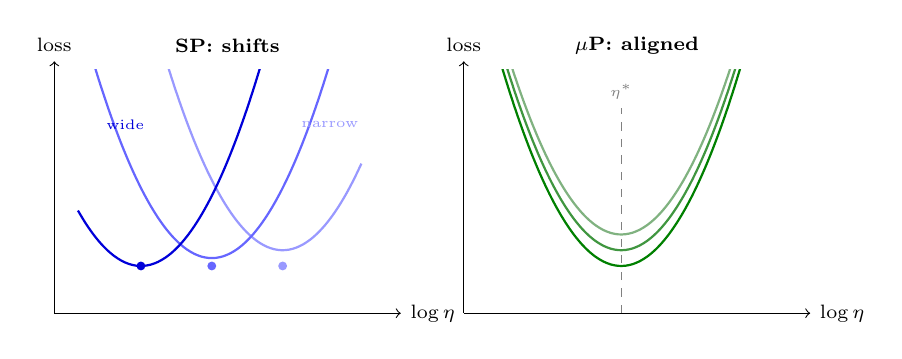
\begin{tikzpicture}
        % SP plot
        \begin{scope}
          \draw[->] (0,0) -- (4.4,0) node[right, font=\scriptsize] {$\log \eta$};
          \draw[->] (0,0) -- (0,3.2) node[above, font=\scriptsize] {loss};
          \node[font=\scriptsize\bfseries] at (2.2,3.4) {SP: shifts};
          \begin{scope}
            \clip (0,0) rectangle (4.3,3.1);
            \draw[blue!40, thick] plot[smooth,domain=0.3:3.9,samples=40] (\x,{0.8+1.1*(\x-2.9)*(\x-2.9)});
            \draw[blue!60, thick] plot[smooth,domain=0.3:3.9,samples=40] (\x,{0.7+1.1*(\x-2.0)*(\x-2.0)});
            \draw[blue!85!black, thick] plot[smooth,domain=0.3:3.9,samples=40] (\x,{0.6+1.1*(\x-1.1)*(\x-1.1)});
          \end{scope}
          \foreach \x/\c in {2.9/blue!40,2.0/blue!60,1.1/blue!85!black} \fill[\c] (\x,{0.6+0*\x}) circle (1.6pt);
          \node[font=\tiny,blue!85!black] at (0.9,2.4) {wide};
          \node[font=\tiny,blue!40] at (3.5,2.4) {narrow};
        \end{scope}
        % muP plot
        \begin{scope}[shift={(5.2,0)}]
          \draw[->] (0,0) -- (4.4,0) node[right, font=\scriptsize] {$\log \eta$};
          \draw[->] (0,0) -- (0,3.2) node[above, font=\scriptsize] {loss};
          \node[font=\scriptsize\bfseries] at (2.2,3.4) {$\mu$P: aligned};
          \begin{scope}
            \clip (0,0) rectangle (4.3,3.1);
            \draw[green!40!black!50, thick] plot[smooth,domain=0.3:3.9,samples=40] (\x,{1.0+1.1*(\x-2.0)*(\x-2.0)});
            \draw[green!45!black!75, thick] plot[smooth,domain=0.3:3.9,samples=40] (\x,{0.8+1.1*(\x-2.0)*(\x-2.0)});
            \draw[green!50!black, thick] plot[smooth,domain=0.3:3.9,samples=40] (\x,{0.6+1.1*(\x-2.0)*(\x-2.0)});
          \end{scope}
          \draw[dashed,gray] (2.0,0) -- (2.0,2.6);
          \node[font=\tiny,gray,anchor=south] at (2.0,2.6) {$\eta^*$};
        \end{scope}
      \end{tikzpicture}%
      }
      \end{center}
      {\scriptsize Loss vs.\ LR for several widths. SP: optimum drifts; $\mu$P: shared optimum $\eta^*$.}
    \end{column}
  \end{columns}
\end{frame}

% -----------------------------------------------------------------------
\begin{frame}{$\mu$P: A Central-Limit Argument at Initialization}

  A hidden preactivation is a \emph{sum over the $n$ input coordinates}:
  \[
    z_j = \sum_{i=1}^{n} W_{ji}\, x_i
  \]

  \begin{itemize}
    \item At init the $W_{ji}$ are i.i.d.\ (mean $0$, variance $\sigma^2$) and independent of the inputs $x_i = \Theta(1)$.
    \item \textbf{Independent terms} $\Rightarrow$ central limit theorem: $\;z_j \xrightarrow{d} \mathcal{N}\!\big(0,\; n\,\sigma^2\,\overline{x^2}\big)$, so $|z_j| = \Theta(\sqrt{n}\,\sigma)$.
    \item \textbf{Desideratum 1 (stable init):} keep $z_j = \Theta(1)$ at \emph{every} width $\;\Rightarrow\; \sigma^2 = \tfrac{1}{n} = 1/\texttt{fan\_in}$.
    \item A width-independent $\sigma^2$ instead gives $|z_j| \sim \sqrt{n} \to \infty$: logits saturate and wider models break.
  \end{itemize}
\end{frame}

% -----------------------------------------------------------------------
\begin{frame}{$\mu$P: A Central-Limit Argument During Training}

  \textbf{Question:} how must the learning rate scale with width so that one step changes the features by a useful, $\Theta(1)$ amount? Apply the same counting to the feature update:
  \[
    \Delta z_j = \sum_{i=1}^{n} \Delta W_{ji}\, x_i
  \]

  \begin{columns}[T]
    \begin{column}{0.54\textwidth}
      \begin{enumerate}
        \item \textbf{The signs are now correlated.} At init the terms were independent, so they \emph{cancelled} ($\sqrt n$). But $\Delta W_{ji}$ is computed \emph{from} $x_i$, so they \emph{align} and \emph{reinforce}: the sum grows like $n$.
        \item If each weight moves by a typical amount $\delta$, this coherent sum gives $\Delta z_j \approx n\,\delta$.
        \item \textbf{We want $\Delta z_j = \Theta(1)$} (features move, but do not explode): $\;n\,\delta = \Theta(1) \Rightarrow \delta = \Theta(1/n)$.
        \item Adam scales every coordinate's step to $\approx \eta$, so $\delta \approx \eta$ and
        \[
          \boxed{\ \eta_{\text{hidden}} \propto 1/n\ }
        \]
      \end{enumerate}
    \end{column}
    \begin{column}{0.44\textwidth}
      \begin{center}
      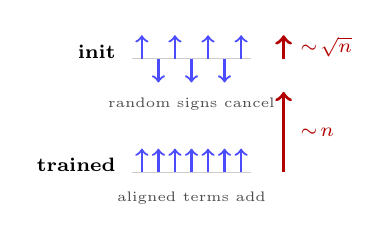
\begin{tikzpicture}[scale=0.6, arr/.style={->, thick, blue!70}]
        % Row 1: init, random signs -> cancel
        \node[font=\scriptsize\bfseries, anchor=east] at (-0.15,0.15) {init};
        \draw[gray!40] (0,0) -- (2.5,0);
        \draw[arr] (0.2,0)--(0.2,0.5);   \draw[arr] (0.55,0)--(0.55,-0.5);
        \draw[arr] (0.9,0)--(0.9,0.5);   \draw[arr] (1.25,0)--(1.25,-0.5);
        \draw[arr] (1.6,0)--(1.6,0.5);   \draw[arr] (1.95,0)--(1.95,-0.5);
        \draw[arr] (2.3,0)--(2.3,0.5);
        \node[font=\tiny, gray!60!black] at (1.25,-0.95) {random signs cancel};
        \draw[->, very thick, red!70!black] (3.2,0)--(3.2,0.5);
        \node[font=\scriptsize, red!70!black, anchor=west] at (3.35,0.25) {$\sim\!\sqrt n$};
        % Row 2: trained, aligned -> add
        \begin{scope}[shift={(0,-2.4)}]
          \node[font=\scriptsize\bfseries, anchor=east] at (-0.15,0.15) {trained};
          \draw[gray!40] (0,0) -- (2.5,0);
          \foreach \x in {0.2,0.55,0.9,1.25,1.6,1.95,2.3} \draw[arr] (\x,0)--(\x,0.5);
          \node[font=\tiny, gray!60!black] at (1.25,-0.55) {aligned terms add};
          \draw[->, very thick, red!70!black] (3.2,0)--(3.2,1.7);
          \node[font=\scriptsize, red!70!black, anchor=west] at (3.35,0.85) {$\sim\! n$};
        \end{scope}
      \end{tikzpicture}
      \end{center}
      {\scriptsize This is the \emph{maximal} stable rate: any larger and $\Delta z_j$ explodes; much smaller is the NTK / lazy limit, where features barely move.}
    \end{column}
  \end{columns}
\end{frame}

% -----------------------------------------------------------------------
\begin{frame}{$\mu$P: Scaling Rules}

  \textbf{Recipe} (relative to standard init, in terms of each matrix's \texttt{fan\_in}/\texttt{fan\_out}; from Table 3 of~\cite{yang2022muP}):

  \vspace{0.3em}
  \begin{center}
    \renewcommand{\arraystretch}{1.35}
    \begin{tabular}{lccc}
      \toprule
      & \textbf{Input \& biases} & \textbf{Hidden} & \textbf{Output / readout} \\
      \midrule
      Init.\ variance & $1/\texttt{fan\_in}$ & $1/\texttt{fan\_in}$ & $1/\texttt{fan\_in}^2$ \\
      SGD LR & $\texttt{fan\_out}\;(\propto n)$ & $1$ & $1/\texttt{fan\_in}\;(\propto 1/n)$ \\
      Adam LR & $1$ & $1/\texttt{fan\_in}\;(\propto 1/n)$ & $1/\texttt{fan\_in}\;(\propto 1/n)$ \\
      \bottomrule
    \end{tabular}
  \end{center}

  \vspace{0.3em}
  \begin{columns}[T]
    \begin{column}{0.5\textwidth}
      \textbf{Reading it (Adam, the LLM case):}
      \begin{itemize}
        \item Embeddings: LR constant in $n$
        \item Hidden \& readout: LR $\propto 1/n$ (shrinks with width)
        \item Readout init $\propto 1/n^2$ (vs.\ $1/n$ in SP): outputs start near zero
      \end{itemize}
    \end{column}
    \begin{column}{0.48\textwidth}
      \textbf{Two more $\mu$P details:}
      \begin{itemize}
        \item \textbf{Attention:} score $= q^\top k / d$, i.e.\ $1/d$ scaling, \emph{not} $1/\sqrt{d}$
        \item \textbf{Output multiplier:} scale logits by $\alpha_{\text{out}}/n$ (a tunable constant)
      \end{itemize}
      {\scriptsize Since $\texttt{fan\_in}=n$ for hidden layers, ``$1/\texttt{fan\_in}$'' $=$ ``$1/n$''.}
    \end{column}
  \end{columns}
\end{frame}

% -----------------------------------------------------------------------
\begin{frame}{$\mu$Transfer: Procedure, Transfer, and Results}

  \begin{columns}[T]
    \begin{column}{0.5\textwidth}
      \textbf{$\mu$Transfer procedure:}
      \begin{enumerate}
        \item Put the model in $\mu$P (per the table)
        \item Tune HPs on a small \emph{proxy} (narrow / shallow, e.g.\ 40M params)
        \item Copy the HPs to the full-scale target: \emph{zero-shot}, no retuning
      \end{enumerate}

      \vspace{0.3em}
      \textbf{Transfers across:} width (primary), and empirically depth (pre-LN), batch size, sequence length, and training time.

      \vspace{0.3em}
      \textbf{HPs that transfer:} learning rate, momentum, Adam $\beta_1,\beta_2$, init variance, LR-schedule shape, attention scale, per-layer multipliers.

      \vspace{0.2em}
      \textbf{Do \emph{not} transfer:} regularization HPs (dropout, weight decay): they depend on model \emph{and} data size, not just width.
    \end{column}
    \begin{column}{0.48\textwidth}
      \textbf{Empirical results:}
      \begin{itemize}
        \item \textbf{GPT-3 6.7B:} HPs tuned on a 40M proxy ($\sim$168$\times$ smaller); tuning cost $\approx$7\% of one pretraining run. Beat the published 6.7B model, matching the 13B model.
        \item \textbf{BERT-large 350M:} tuned from a 13M proxy; total tuning cost $\approx$ one BERT-large pretraining, and \emph{beat} published BERT-large.
        \item \textbf{``Wider is better''} holds throughout training under $\mu$P, unlike SP.
      \end{itemize}

      \vspace{0.3em}
      \textbf{Caveats:} depth transfer is more fragile than width; interacts with normalization/residual scaling; regularization still needs tuning at scale. Adopted by Cerebras-GPT and several LLM labs.
    \end{column}
  \end{columns}
\end{frame}

% -----------------------------------------------------------------------
\subsection{LLM Training Recipes}

% -----------------------------------------------------------------------
\begin{frame}{LLM Hyperparameter Recipes}

  \begin{center}
    \renewcommand{\arraystretch}{1.2}
    \resizebox{\textwidth}{!}{%
    \begin{tabular}{lccccccc}
      \toprule
      & \textbf{GPT-3} & \textbf{Chinchilla} & \textbf{LLaMA} & \textbf{LLaMA-2} & \textbf{LLaMA-3} & \textbf{DeepSeek-V3} \\
      & \scriptsize 175B & \scriptsize 70B & \scriptsize 65B & \scriptsize 70B & \scriptsize 405B & \scriptsize 671B (MoE) \\
      \midrule
      Peak LR & $6 \times 10^{-5}$ & $1 \times 10^{-4}$ & $1.5 \times 10^{-4}$ & $1.5 \times 10^{-4}$ & $8 \times 10^{-5}$ & $2.2 \times 10^{-4}$ \\
      LR schedule & cosine & cosine & cosine & cosine & cosine & WSD \\
      Min LR & $10\%$ of peak & $10\%$ of peak & $10\%$ of peak & $10\%$ of peak & $\frac{1}{80}$ peak & $\frac{1}{10}$ peak \\
      Warmup & 375M tok & 5B tok & 2000 steps & 2000 steps & 8000 steps & 2000 steps \\
      Batch size (tok) & 3.2M & 1.5M & 4M & 4M & 16M & 15.6M \\
      Weight decay & 0.1 & 0.1 & 0.1 & 0.1 & 0.1 & 0.1 \\
      $\beta_1, \beta_2$ & 0.9, 0.95 & 0.9, 0.95 & 0.9, 0.95 & 0.9, 0.95 & 0.9, 0.95 & 0.9, 0.95 \\
      Grad clip & 1.0 & 1.0 & 1.0 & 1.0 & 1.0 & 1.0 \\
      Tokens trained & 300B & 1.4T & 1.4T & 2T & 15T & 14.8T \\
      Tok / param ratio & 1.7 & 20 & 21.5 & 28.6 & 37 & 22.1 \\
      \bottomrule
    \end{tabular}%
    }
  \end{center}

  \vspace{0.2em}
  {\small Sources: \cite{brown2020gpt3}, \cite{hoffmann2022chinchilla}, \cite{touvron2023llama}, \cite{touvron2023llama2}, \cite{grattafiori2024llama3}, \cite{deepseekai2024deepseekv3}.}
\end{frame}

% -----------------------------------------------------------------------
\begin{frame}{Common Patterns in LLM Recipes}

  Remarkably, despite different model sizes and labs, most choices converge:

  \vspace{0.4em}
  \textbf{Near-universal defaults:}
  \begin{itemize}
    \item \textbf{Optimizer:} AdamW with $\beta_1 = 0.9$, $\beta_2 = 0.95$
    \item \textbf{Weight decay:} $\lambda = 0.1$
    \item \textbf{Gradient clipping:} global norm $= 1.0$
    \item \textbf{LR schedule:} cosine decay (WSD emerging as alternative)
    \item \textbf{Precision:} BF16 mixed precision
  \end{itemize}

  \vspace{0.4em}
  \textbf{Model-size-dependent:}
  \begin{itemize}
    \item \textbf{Peak learning rate:} Decreases with model size. Roughly $\eta \propto N^{-0.1}$ to $N^{-0.2}$
    \item \textbf{Batch size:} Increases with model size (to match $B_{\text{crit}}$)
    \item \textbf{Warmup steps:} Relatively short ($\sim$0.1--1\% of training)
  \end{itemize}

  \vspace{0.4em}
  \textbf{Trend:} Labs are now training \emph{far beyond} Chinchilla-optimal token counts.
  Inference cost matters: a smaller model trained on more data is cheaper to \emph{serve}.
\end{frame}

% -----------------------------------------------------------------------
\begin{frame}{Vision Model Hyperparameter Recipes}

  \begin{center}
    \renewcommand{\arraystretch}{1.15}
    \resizebox{\textwidth}{!}{%
    \begin{tabular}{lccccccc}
      \toprule
      & \textbf{ResNet-50} & \textbf{ResNet-50} & \textbf{ResNeXt-101} & \textbf{ViT-B/16} & \textbf{ViT-L/16} & \textbf{MAE} & \textbf{DINOv2} \\
      & \scriptsize orig. & \scriptsize improved & & & & \scriptsize ViT-L & \scriptsize ViT-L/14 \\
      \midrule
      Optimizer & SGD+mom & LAMB & SGD+mom & Adam & Adam & AdamW & AdamW \\
      Peak LR & 0.1 & $5 \times 10^{-3}$ & 0.1 & $8 \times 10^{-4}$ & $4 \times 10^{-4}$ & $1.5 \times 10^{-4}$ & $2 \times 10^{-4}$ \\
      LR schedule & step & cosine & step & lin.\ decay & lin.\ decay & cosine & cosine \\
      Warmup & --- & 5 ep & --- & 10k steps & 10k steps & 40 ep & 80 ep \\
      Batch size & 256 & 2048 & 256 & 4096 & 4096 & 4096 & $\sim$1024 \\
      Weight decay & $10^{-4}$ & 0.02 & $10^{-4}$ & 0.1 & 0.1 & 0.05 & 0.04$\to$0.4 \\
      $\beta_1, \beta_2$ & 0.9, -- & -- & 0.9, -- & .9, .999 & .9, .999 & .9, .95 & .9, .999 \\
      Grad clip & --- & --- & --- & 1.0 & 1.0 & --- & 3.0 \\
      Epochs & 90 & 600 & 100 & 7 (JFT) & 7 (JFT) & 800 & 500 \\
      Resolution & 224 & 224 & 224 & 224 & 224 & 224 & 224 \\
      \bottomrule
    \end{tabular}%
    }
  \end{center}

  \vspace{0.3em}
  {\small \textbf{Trends:} Vision moved from SGD (ResNet era) $\to$ AdamW (ViT era). Modern recipes use cosine LR, longer training, heavier augmentation, and much larger batches.}

  {\scriptsize Sources: \cite{he2016resnet}, \cite{wightman2021resnet}, \cite{xie2017resnext}, \cite{dosovitskiy2021vit}, \cite{he2022mae}, \cite{oquab2023dinov2}.}
\end{frame}

% -----------------------------------------------------------------------
\begin{frame}{Contrastive \& Multimodal Model Recipes}

  \begin{center}
    \renewcommand{\arraystretch}{1.15}
    \begin{tabular}{lccc}
      \toprule
      & \textbf{CLIP ViT-L/14} & \textbf{SigLIP} & \textbf{PaliGemma} \\
      & \scriptsize OpenCLIP repro. & & \\
      \midrule
      Optimizer & AdamW & Adafactor & Adafactor \\
      Peak LR & $5 \times 10^{-4}$ & $10^{-3}$ & rsqrt schedule \\
      LR schedule & cosine & cosine & rsqrt (continuous) \\
      Warmup & 2000 steps & 200M examples & slow linear \\
      Batch size & 32,768 & 32,768 & --- \\
      Weight decay & 0.2 & $10^{-4}$ & --- \\
      $\beta_1, \beta_2$ & .9, .98 & .9, .95 & --- \\
      Training data & 400M pairs & 40B examples & 1B examples \\
      Resolution & 224 & 224 & 224$\to$448/896 \\
      \bottomrule
    \end{tabular}
  \end{center}

  \vspace{0.3em}
  {\small \textbf{Key differences from LLMs:}
  \begin{itemize}
    \item Contrastive models need very large batch sizes (32k+) for enough negatives
    \item SigLIP replaces softmax cross-entropy with sigmoid loss $\Rightarrow$ scales better to huge batches
    \item Weight decay varies widely: 0.2 (CLIP) vs.\ $10^{-4}$ (SigLIP). Less converged than LLM recipes
    \item Multimodal models often use multi-stage training with increasing resolution
  \end{itemize}
  }

  {\scriptsize Sources: \cite{radford2021clip}, \cite{zhai2023siglip}, \cite{beyer2024paligemma}.}
\end{frame}

% -----------------------------------------------------------------------
\subsection{Practical Guidelines}

% -----------------------------------------------------------------------
\begin{frame}{Practical Hyperparameter Selection Workflow}

  \textbf{Recipe for practitioners:}

  \vspace{0.4em}
  \begin{enumerate}
    \item \textbf{Start from published recipes.} Use HP settings from a similar published model as a baseline (see previous table).

    \item \textbf{Tune learning rate first.} It has the largest impact. Use:
      \begin{itemize}
        \item LR range test for a quick estimate
        \item Small grid: $\{1, 3, 5\} \times 10^{k}$ for 2--3 orders of magnitude
      \end{itemize}

    \item \textbf{Use $\mu$P for large models.} Tune on a small proxy ($\sim$$10\text{--}100\times$ cheaper), transfer LR and other HPs to the target scale.

    \item \textbf{Keep everything else at defaults.} Weight decay $= 0.1$, $\beta_1 = 0.9$, $\beta_2 = 0.95$, grad clip $= 1.0$.

    \item \textbf{Use short runs for exploration.} Train for 1--5\% of total budget to compare configurations. Scaling laws can extrapolate final performance.

    \item \textbf{Monitor loss curves.} Watch for spikes (reduce LR or increase warmup), slow convergence (increase LR), or late divergence (add grad clipping).
  \end{enumerate}
\end{frame}


